\chapter{Square cylinder}

\begin{figure}[h]
	\begin{subfigure}{\textwidth}
		\centering
		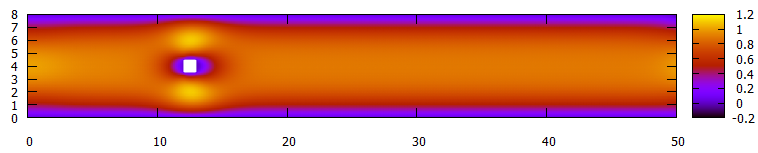
\includegraphics[width=.8\linewidth]{Square/totu1}
		\caption{$Re=1$}
	\end{subfigure}
	\begin{subfigure}{\textwidth}
		\centering
		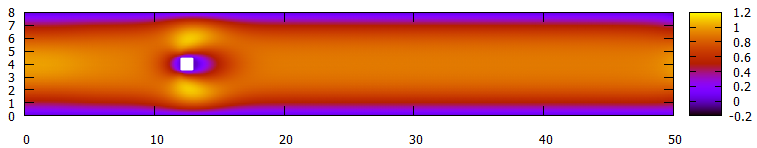
\includegraphics[width=.8\linewidth]{Square/totu3}
		\caption{$Re=3$}
	\end{subfigure}
	\begin{subfigure}{\textwidth}
		\centering
		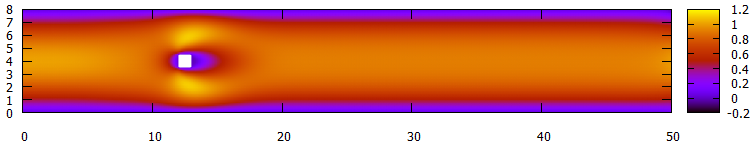
\includegraphics[width=.8\linewidth]{Square/totu5}
		\caption{$Re=5$}
	\end{subfigure}
	\begin{subfigure}{\textwidth}
		\centering
		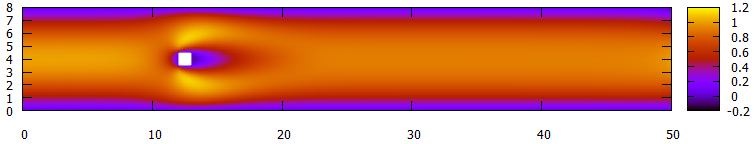
\includegraphics[width=.8\linewidth]{Square/totu10}
		\caption{$Re=10$}
	\end{subfigure}
	\begin{subfigure}{\textwidth}
		\centering
		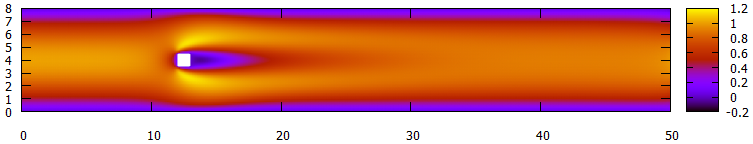
\includegraphics[width=.8\linewidth]{Square/totu30}
		\caption{$Re=30$}
	\end{subfigure}
	\begin{subfigure}{\textwidth}
		\centering
		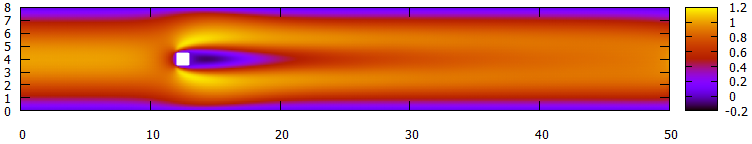
\includegraphics[width=.8\linewidth]{Square/totu50}
		\caption{$Re=50$}
	\end{subfigure}
\caption{Horizontal velocity in the channel}
\end{figure}

\begin{figure}[h]
	\begin{subfigure}{\textwidth}
		\centering
		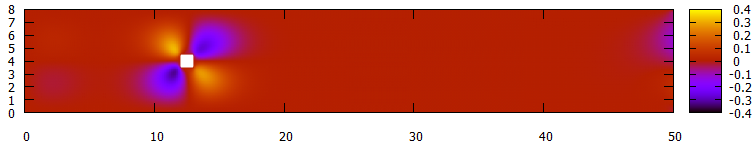
\includegraphics[width=.8\linewidth]{Square/totv1}
		\caption{$Re=1$}
	\end{subfigure}
	\begin{subfigure}{\textwidth}
		\centering
		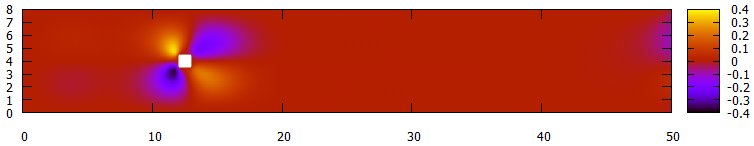
\includegraphics[width=.8\linewidth]{Square/totv3}
		\caption{$Re=3$}
	\end{subfigure}
	\begin{subfigure}{\textwidth}
		\centering
		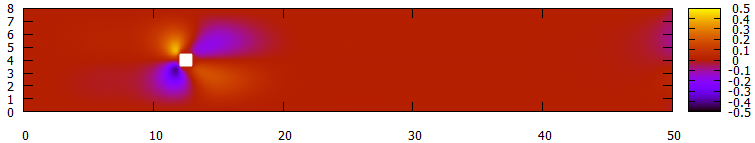
\includegraphics[width=.8\linewidth]{Square/totv5}
		\caption{$Re=5$}
	\end{subfigure}
	\begin{subfigure}{\textwidth}
		\centering
		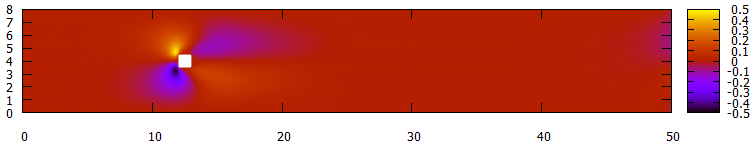
\includegraphics[width=.8\linewidth]{Square/totv10}
		\caption{$Re=10$}
	\end{subfigure}
	\begin{subfigure}{\textwidth}
		\centering
		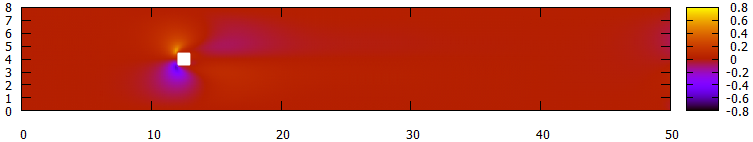
\includegraphics[width=.8\linewidth]{Square/totv30}
		\caption{$Re=30$}
	\end{subfigure}
	\begin{subfigure}{\textwidth}
		\centering
		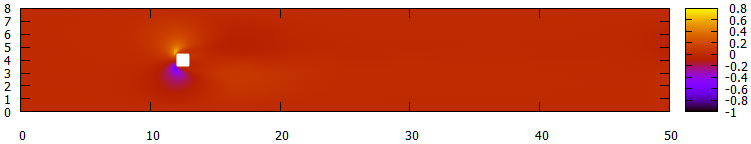
\includegraphics[width=.8\linewidth]{Square/totv50}
		\caption{$Re=50$}
	\end{subfigure}
	\caption{Vertical velocity in the channel}
\end{figure}